\section{Literature}

The IPE literature on the relationship between politics and FDI has focused largely on how political factors shape and direct the flow of FDI across countries. Among the considered factors include: corruption, regime type, political violence, expropriation, etc. The dominant theoretical insight in this literature is the ``obsolescing bargain'' power of foreign firms. Once foreign firms sink their illiquid investment into the host countries, they no longer have a bargaining power and may be vulnerable to the caprice and avarice of the host. All of the political factors are a variant on what characteristics of the state mitigate or exacerbate this obsolescing bargaining problem.  Later analyses extend the framework to dyadic framework, examining the interplaying effect of both the host and the home country characteristics.

Is this interesting? Presumably it is interesting because we care about the role of the nation states in the international economy, which in turn it is important because the flow of FDI has welfare implications for millions of citizens in the host countries. A frequent policy conclusion from this body of research is echoed widely in the policy sphere is that countries need to improve the investment climate, reduce corruption, or maintain political stability to attract FDI.

But do countries want to? This causally prior question, and arguably more pregnant with politics, it has been understudied. 

On the one hand, some scholars have looked at the demand for FDI. However, these efforts have been stymied by recalcitrant issues with data and methods.

One the other hand, I also want to raise the issue of the quality of FDI.

Implicit in this phrase are two under-examined ideas: one is that country always want to attract FDI. Two is that it does not differentiate between the type of FDI that a country would want.

\section{The need for a new model}

Summarize the problems

To deal with this problem, I adopt the two-sided matching approach, previously used in the labor market and marriage market. This approach will be able to solve the above problems in several ways.

\subsection{Measuring Multinational Corporations' Activities}

For most of political science theory regarding FDI, we ultimately care about the scale of multinationals' activities in a country, and not necessarily about how much FDI has crossed through its border. Indeed, we theorize about how multinationals may reduce their activities for fear of expropriation, and how the host country's political factors can induce multinationals to invest more with a credible commitment not to expropriate. It is also the scale of multinationals' activities that determines how many jobs are created or how much of the domestic market is competed away, engendering labor's support and local business' lament.

To measure the scale of multinationals' activities, the vast majority of political science works uses FDI stock and flow \citep{Jensen2003, Ahlquist2006, Beazer2011, Graham2010}. However, as \citet{Kerner2014} points out, these measures, whose original purpose is to monitor balance of payments, are often misleading about multinationals' activities. FDI flow do not count locally raised capital and reinvested earnings since they do not cross any border. FDI stock calculated at market value fluctuates based on market price, unrelated to firms' behavior. FDI stock calculated at historical value, which records asset value at the time it was acquired, is more stable and appropriate to measure the scale of MNCs' activities. However, due to the onerous data requirements, most countries measures FDI stock by simply adding up FDI flow across years.

Given the interest of political science theory in MNCs' activities, \citet{Kerner2014} suggests less use of FDI stock and flow and more use of firm-level statistics. While firm-level data has become more abundant in recent years,\footnote{Examples of firm-level data include the US Bureau of Economic Analysis (BEA)'s survey of all US firms abroad, Tokyo Keizai's Overseas Japanese companies database (\textit{Kaigai Sinshutsu Kigyou Souran}), World Bank's Enterprise Survey, and Orbis database of companies worldwide.} appropriate methods have not been developed. Given the data structure of a set of firms investing in a set of countries, one may consider a dyadic-based analysis, frequently used in the International Relations literature. In such analysis, the unit of observation is a firm-country dyad, and the model used is typically an OLS regression. Each dyad is assumed to be independent of each other, and any bias due to interdependency between dyads is fixed via post-estimation procedures, such as clustered standard errors \citep{Dorff2013}. 

However, this approach would be inappropriate to analyze MNCs' investment location. Once a firm chooses to invest in a country, it is by definition not investing in another country. Therefore, firm-country dyads deterministically constrained one another and cannot be modeled as independent draws from a common distribution.

The two-sided matching model would be able to deal with this problem.


\subsection{Estimating Countries' Demand for FDI}

Recognizing the need to theorize about the demand for FDI, scholars have recently paid more attention to this area \citep{Pinto2013, Pandya2016}. Similar to the rich IPE literature in trade and exchange rate \citep{Broz2001, Milner2005a}, these studies argue that countries' demand for FDI varies according to FDI's distributive effect on their domestic constituencies.\footnote{The alternative to preference as the explanan of FDI flow is institutional characteristics.} In this theoretical framework, labor supports FDI because foreign firms bring capital that increases the demand for labor and raises productivity, both of which lead to higher wage. On the other hand, domestic firms oppose FDI because foreign firms compete with them for labor, local inputs, and markets. Both \citet{Pinto2013} and \citet{Pandya2016} formulate their theories as a variant of this labor-vs-business tension, which surfaces in the former work as left-vs-right governments, and in the latter as democratic-vs-authoritarian regimes.

While these pioneering works have enriched our understanding of the relationship between politics and FDI, serious empirical issues prevent their statistical analyses from truly validating their theoretical arguments. The bottleneck is measuring country's demand for FDI.

For example, consider \citet{Pinto2008, Pinto2013}'s approach, which controls for economic and institutional factors that affect bilateral FDI flow into a country. The author then claims that the country's demand for FDI is what's left in the residual.\footnote{Specifically, the estimation of FDI openness involves two steps. First, the author runs a gravity model explaining bilateral FDI flows, estimating the intercept as the host country-year fixed effect. Second, this fixed effect is then regressed on several economic and endowment factors of that country-year (i.e. GDP, GDP per capita, average school years, arable land). The residual of the second stage is considered the country's ``FDI openness'' in that year.} For this approach to be valid, every economic, institutional, and endowment factors that affect FDI flow have to be controlled for, leaving only the country's demand in the error term. This claim is much stronger than the regular assumption of exogenous and normally distributed error, which is valid as long as the omitted factors are uncorrelated with the independent variable of interest. Framed substantively, since the residual is likely to contain more than just the country's demand for FDI, if we observe an abnormally high level of FDI we still do not know whether it is because the country welcomes FDI or because foreign firms find something attractive in the country.\footnote{In addition, the data requirement of bilateral FDI flows, ideally disaggregated by sectors, is very demanding. Therefore, this approach is limited to OECD countries only \citep{Pinto2008}. During the period the authors study, 1980-2000, OECD countries accounted for 95\% of global FDI outflow and 90\% of inflow. However, since then the role of the developed world in global FDI has declined sharply, reduced to 60.8\% of outflow and 40.6\% of inflow in 2014 \citep{UNCTAD2015}.}

In contrast to \citet{Pinto2013}'s statistical approach, \citet{Pandya2014, Pandya2016} aimed to substantively measure countries' demand for FDI, using the annual US Investment Climate Reports to code how many industries have foreign ownership restriction or face investment screening. This measurement is easier to interpret and available for many countries. However, two problems remain. First, adding up the raw count of restricted industries is not appropriate because industries are not all the same. For example, given the reach of the banking sector into all corners of the economy, a country's opening up its financial industry indicates much more FDI-friendliness than, say, allowing foreign furniture makers to set up shops. Since the theoretical argument is driven by FDI's distributive effect, it is suspect to ignoring the varying effect of FDI across sectoral constituencies. Second, given the coding rules, an industry is coded as free if there is no mention of restriction. If the industry in a FDI receives little FDI, it may not be worth mentioning, and yet still coded as open. Thus, where there is little FDI it may look like the country is extremely friendly. This concern is not hypothetical. \Cref{fig:china_fdi_restriction} shows that, following the coding of the US Investment Climate Reports, China seemed to be 100\% open to FDI up until 1986, when it started imposing restrictions. The reality is opposite. When China first opened up for FDI in 1979, only limited FDI is allowed as joint-venture in Special Economic Zones (SEZ). The year of 1986 was, in fact, the first time China allowed any wholly owned FDI outside of SEZs.

\begin{figure}[!ht]
\centering
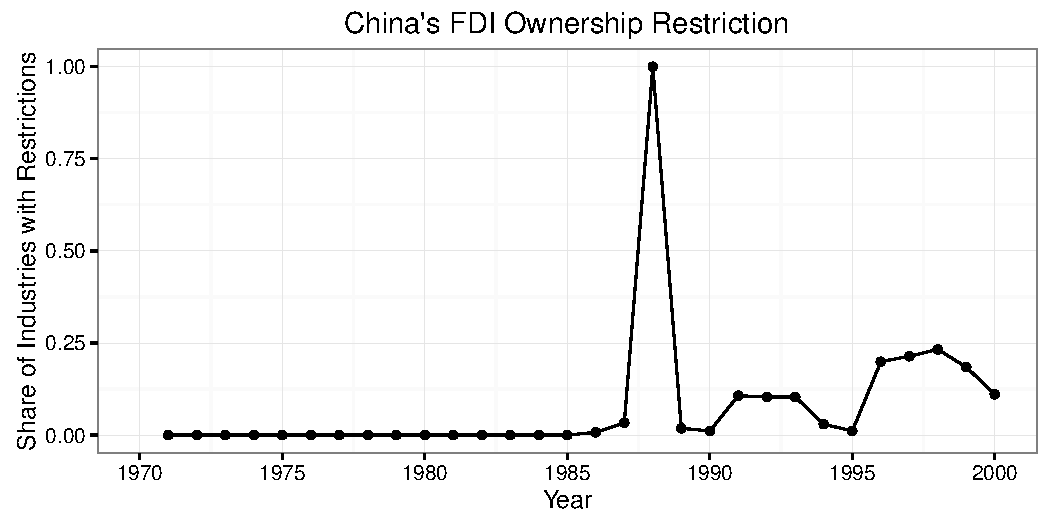
\includegraphics[width=0.75\textwidth,keepaspectratio]{../figure/china_fdi_restriction}
\caption{China's FDI Ownership Restriction, as coded in \citet{Pandya2010}. The sharp spike in 1988 also does not seem to correspond to any actual change in policy, and thus likely an artifact of reporting. See \citet{Zebregs2002} for a historical overview of China's FDI policy.}
\label{fig:china_fdi_restriction}
\end{figure}



\subsection{Countries' preference for specific FDI characteristics}

This section talks about the need to look at different types of MNCs.

While political science literature has focused almost exclusively on the quantity of FDI, treatment all FDI as a homogeneous flow of capital, policy makers seem to pay much more attention to distinguishing types of FDI. Commenting on the role of International Investment Agreements (IIAs), \citet{UNCTAD2015} says, ``Today, increasing the quantity of investment is not enough. What matters is its quality, i.e. the extent to which investment delivers concrete sustainable development benefits.'' Governments from Ireland, Ghana, to China all offer various forms of tax incentives and fee waivers to attract FDI that invests in a remote region, brings new technology, or focuses on exporting \citep{Ricupero2000}. Since 2006, China's official FDI policy has been ``quality over quantity,'' promoting FDI with intense R\&D and in high-productivity sectors \citep{Guangzhou2011}.\footnote{All of these models also cannot investigate countries' preference for specific firms' characteristics. Pondya's look at cross industry, but because of data issue she can only do cross-sectional at the industry level instead of country-industry level. This level of aggregation is dubious: the same industry in one country is different from another country. For example, automobile value chain is vastly different across countries (example here). All of the industry estimates are based on US firms, which really cannot be realized to others. (It can for some basic industry characteristics / technology level, not for whether an industry is market oriented or not.)}

Disaggregating FDI has been a very difficult task. The few existing attempts can only use detailed data from one country or limit the sample to OECD countries \citep{Alfaro2003, Alfaro2007, Javorcik2004}. Using firm level data, this is not as challenging, but brings up the need for an appropriate model.

